\documentclass[12pt]{report}
\usepackage[T1]{fontenc}
\usepackage[utf8]{inputenc}
\usepackage[francais]{babel}
\usepackage{amsmath}
\usepackage{amsfonts}
\usepackage{amssymb}
\usepackage{fancybox}
\usepackage{fancyhdr}
\usepackage{amsthm}
\usepackage{mathrsfs}
\usepackage{fix-cm}
\usepackage{graphicx}
\usepackage{caption}
\usepackage{subcaption}
\usepackage{textcomp}
\usepackage{lmodern}
\usepackage[tikz]{bclogo}
\usepackage{color}
\usepackage{lipsum}
\usepackage{hyperref}
\usepackage[Glenn]{fncychap}
\usepackage{float}
\usepackage{listings}
\usepackage{enumerate}
\usepackage[strict]{changepage}
\usepackage{ragged2e}
\usepackage{lmodern}
\usepackage{lastpage}
\usepackage{systeme}
\usepackage{listings}
\usepackage{xcolor}
\usepackage{textcomp}

\lstset{upquote=true,
	columns=flexible,
	keepspaces=true,
	breaklines,
	breakindent=0pt,
	basicstyle=\ttfamily,
	commentstyle=\color{green!60!black},
	language=Scilab,
	alsoletter=\),
	classoffset=0,
	keywordstyle=\color{violet!75},
	deletekeywords={zeros,disp,plot2d,clf},
	classoffset=1,
	keywordstyle=\color{cyan},
	morekeywords={zeros,disp,plot2d},
	classoffset=2,
	keywordstyle=\color{violet!75},
	morekeywords={clf, clc},
	classoffset=3,
	keywordstyle=\color{magenta!70!pink!50!},
	morekeywords={\%f, \%t, \%pi},
	extendedchars=true,
	showstringspaces=false,
	otherkeywords={\%f, \}, \{, \&, \|},
	literate={0}{{\color{brown!75}0}}1 
	{1}{{\color{brown!75}1}}1 
	{2}{{\color{brown!75}2}}1 
	{3}{{\color{brown!75}3}}1 
	{4}{{\color{brown!75}4}}1 
	{5}{{\color{brown!75}5}}1 
	{6}{{\color{brown!75}6}}1 
	{7}{{\color{brown!75}7}}1 
	{8}{{\color{brown!75}8}}1 
	{9}{{\color{brown!75}9}}1 
	{(}{{\color{blue!50}(}}1
	{)}{{\color{blue!50})}}1
	{[}{{\color{blue!50}[}}1
	{]}{{\color{blue!50}]}}1
	{-}{{\color{gray}-}}1
	{+}{{\color{gray}+}}1
	{=}{{\color{gray}=}}1
	{:}{{\color{orange}:}}1
	{à}{{\`a}}1
	{À}{{\`A}}1
	{é}{{\'e}}1
	{è}{{\`e}}1
}

\definecolor{anti-flashwhite}{rgb}{0.95, 0.95, 0.96}
\definecolor{aliceblue}{rgb}{0.94, 0.97, 1.0}
\definecolor{beige}{rgb}{0.96, 0.96, 0.86}
\definecolor{lightapricot}{rgb}{0.99, 0.84, 0.69}
\definecolor{lightkhaki}{rgb}{0.94, 0.9, 0.55}
\definecolor{bisque}{rgb}{1.0, 0.89, 0.77}
\definecolor{arylideyellow}{rgb}{0.91, 0.84, 0.42}
\usepackage[left=2.5cm,right=2.5cm,top=3cm,bottom=2cm]{geometry}


%\renewcommand{\footrulewidth}{1pt}
%\fancyfoot[C]{\textbf{page \thepage}} 
%\fancyfoot[L]{Mémoire SMA S6}
%\fancyfoot[R]{2020-2021}

%\usepackage[frenchb]{babel}
\addto\captionsfrench{\renewcommand{\chaptername}{Partie}}

\author{\ }
\title{\ }
\usepackage{lmodern}
\DeclareUnicodeCharacter{2212}{-}
\begin{document}

  
  \begin{titlepage}
   \begin{sffamily}
    \begin{center}
     
     
     
\includegraphics[scale=0.25]{Lg4.png}~\\
     
\includegraphics[scale=0.55]{Lg5.png}~\\[1.9cm]
     
     \textsc{\LARGE Université de Versailles}\\[0.1cm]
     \textsc{\LARGE Saint-Quentin-en-Yvelines}\\ 
     \textsc{Département de Informatique}\\[1.8cm]
     
    \textsc{\Large Master 1 Calcul Haute Performance, Simulation}\\[1.9cm]
    

     
     \rule{0.75\textwidth}{2pt}\\[0.1cm]
     \emph{\textbf{\large TD/TP - Calcul Numérique}}\\ 
     \rule{0.75\textwidth}{2pt}\\[1.3cm]
     

     \begin{minipage}{0.4\textwidth}
      \begin{flushleft} \large
       \textit{\Large Réalisé par :} \\
       \textsc{\normalsize BOUCHELGA ABDELJALIL}\\
      
       
      \end{flushleft}
     \end{minipage}
     \begin{minipage}{0.4\textwidth}
      \begin{flushright} \large
       \textit{\Large Encadré par :}\\
       \textsc{\normalsize Pr.THOMAS DUFAUD}\\
       
      \end{flushright}
     \end{minipage}\\[1cm]
     
   
     
     \vfill
     

     {\large Année Universitaire:2021-2022}
     
    \end{center}
   \end{sffamily}
  \end{titlepage}
  
%\addcontentsline{toc}{section}{Remerciement}
%\addcontentsline{toc}{section}{Introduction}
%\addcontentsline{toc}{section}{Notations}

\pagebreak
\normalsize
\renewcommand{\footrulewidth}{1pt}


\chapter{Introduction}
L'objectif de TD/TP 2 est de prendre les automatismes sur la rédaction des algorithmes et leur analyse. Pour cela nous allons écrire des algorithmes numérique et évaluer leur complexité arithmétique et en terme de stockage mémoire et puis comparer leurs performances afin d'implémenter des algorithmes efficace en terme de performance.\\

Pour le TD/TP 3 l'objectif est de savoir différentes type d'algorithme de résolution d'un système linéaire, ainsi comprendre les performances et les limites de chaque algorithme et puis comparer les performances.\\

\textbf{Outil utilisé}\\[0.5cm]
1. Scilab\\
2. Latex\\
3. 


\chapter{TD/TP 2 Calcul Numérique}
\section{Exercice 1 TP}
Le but de cet exercice est de se familiariser avec le langage Scilab et savoir les notion basic qu'on aura besoin par la suite. \\[0.4cm]
1. Écrivez un vecteur $x$ à 1 ligne et 4 colonnes.
\begin{lstlisting}[]
-->x=[1,2,3,4]
x  = 

1.   2.   3.   4.
\end{lstlisting}
2. Écrivez un vecteur y à 4 lignes et 1 colonnes
\begin{lstlisting}[]
-->y=[1;2;3;4]
y  = 

1.
2.
3.
4.
\end{lstlisting}
3. les opérations
\begin{lstlisting}[]
-->x=[1;2;3;4]
x  = 

1.
2.
3.
4.

-->z=x+y

z  = 

2.
4.
6.
8.


-->x=[1,2,3,4]
x  = 

1.   2.   3.   4.

-->s=x*y
s  = 

30.
\end{lstlisting}
4. la fonction size() 
\begin{lstlisting}[]
-->size(x)
ans  =

1.   4.

-->size(y)
ans  =

4.   1.
\end{lstlisting}
5. la norme 2 de x avec la fonction norme
\begin{lstlisting}[]
-->norm(x)
ans  =

5.4772256
\end{lstlisting}
6. matrice A à 4 lignes et 3 colonnes
\begin{lstlisting}[]
-->A=[1,2,3;4,5,6;7,8,9;10,11,12]
A  = 

1.    2.    3. 
4.    5.    6. 
7.    8.    9. 
10.   11.   12.
\end{lstlisting}
7. la transposée de A.
\begin{lstlisting}[]
-->A'
ans  =

1.   4.   7.   10.
2.   5.   8.   11.
3.   6.   9.   12.
\end{lstlisting}
8. les opérations de bases avec deux matrices carrées A et B
\begin{lstlisting}[]
-->B=[1,1,1;2,2,2;3,3,3;4,4,4]
B  = 

1.   1.   1.
2.   2.   2.
3.   3.   3.
4.   4.   4.

-->A
A  = 

1.    2.    3. 
4.    5.    6. 
7.    8.    9. 
10.   11.   12.

La somme:

-->c=A+B
c  = 

2.    3.    4. 
6.    7.    8. 
10.   11.   12.
14.   15.   16.

Le produit: 

-->D=A*B'
D  = 

6.    12.   18.   24. 
15.   30.   45.   60. 
24.   48.   72.   96. 
33.   66.   99.   132.

La soustraction: 

-->E=A-B
E  = 

0.   1.   2.
2.   3.   4.
4.   5.   6.
6.   7.   8.
\end{lstlisting}
9. le conditionnement de A avec la fonction cond().
\begin{lstlisting}[]
-->cond(A)
ans  =

9.882D+15
\end{lstlisting}      

\section{Exercice 2 TP : Matrice random et problème "jouet"}
1. Génération d'une matrice A de taille 3 × 3 en utilisant la fonction rand().
\begin{lstlisting}[]
-->A=rand(3,3)
A  = 

0.2113249   0.3303271   0.8497452
0.7560439   0.6653811   0.685731 
0.0002211   0.6283918   0.8782165
\end{lstlisting}  

2. Génération d'un vecteur $xex \in \mathbb{R}$ avec la fonction rand().
\begin{lstlisting}[]
-->xex=rand(1:3)
xex  = 

0.068374   0.5608486   0.6623569

-->xex'
ans  =

0.7263507
0.1985144
0.5442573
\end{lstlisting}  

3. Calcul de $b = A*xex$

\begin{lstlisting}[]
-->b=A*xex
b  = 

0.6815507
1.0544548
0.6028812
\end{lstlisting}  

4. Résolution du système $Ax=b$ avec la fonction $"\backslash"$.
\begin{lstlisting}[]
-->x=A\b
x  = 

0.2320748
0.2312237
0.2164633  
\end{lstlisting}  

\textbf{Remarque :} Lorsque $A$ est carré et non singulière, $x=A\backslash b $ est équivalent à $x=inv(A)*b$ en arithmétique exacte, mais le calcul réalisé par $backslash$ est plus précis et et moins coûteux en arithmétique flottante. Par conséquent, pour calculer la solution du système d'équations linéaires $Ax=b$, on devrait plutôt utiliser l'opérateur $backslash$, et éviter la fonction $inv$ qui numériquement moins stable.\\

5. Calcul de l'erreur avant et arrière \\

Erreur avant :
\begin{lstlisting}[]
-->err_avant=norm(xex-x)/norm(xex)
err_avant  = 

3.999D-16
\end{lstlisting}

Erreur arrière : 
\begin{lstlisting}
-->r=b-A*x
r  = 

0.       
5.551D-17
5.551D-17

-->relres = norm(r)/norm(A)*norm(x)
relres  = 

1.734D-17
\end{lstlisting}

Conditionnement :           
\begin{lstlisting}
-->cond(A)
ans  =

8.2596760 
\end{lstlisting}           
          
6. Test avec differentes tailles\\
Pour refaire les 5 points précedentes j'ai creer le script en desous et à chaque fois je change la taille.  
\begin{lstlisting}

function a=jouet(n)
A=rand(n,n)    //Matrice de taille n
c=cond(A)
disp("c =", c)
xex=rand(1:n)  //Vecteur de taille n
xex=xex'
b=A*xex        //calcul de b
x=A\b          //Resolution du systeme
disp("x = ",x)
err_avant=norm(xex-x)/norm(xex)  //Erreur Avant
disp("Erreur_Avant = ",err_avant)
r=b-A*x                          //Erreur Arriere
disp("r =",r)
relres = norm(r)/(norm(A)*norm(x))
disp("Relres = ",relres)
a=1
endfunction
\end{lstlisting}     

\textbf{Analyse des resultats}\\
Nous remarquons que le conditionnement augmente lorsqu'on augmente la taille de la matrice, ce qui justifier l'augmentation des erreurs arriére et avant, ainsi l'erreur avant est toujour supérieur à l'erreur arriére. 
      
\section{Exercice 2 TP : Produit Matrice-Matrice} 
le but de ce tp est de comparer la complixité de 3 trois algorithme qui font le produit de deux matrices.
         
L’algorithme du produit Matrice-Matrice "ijk" \textbf{matmat3b}
\begin{lstlisting}
function [C]= matmat3b(A,B)
 m=size(A,1);
 p=size(B,1);
 n=size(B,2);
 C=zeros(m,n);
 for i = 1 : m
  for j = 1 : n
   for k = 1 : p
    C(i, j) = A(i, k)*B(k, j) + C(i, j);
   end 
  end 
 end 
endfunction
\end{lstlisting}     

L’algorithme du produit Matrice-Matrice "ijk" \textbf{matmat2b}
\begin{lstlisting} 
function [C]= matmat2b(A,B)
 m=size(A,1);
 n=size(B,2);
 C=zeros(m,n);
 for i = 1 : m
  for j = 1 : n
   C(i, j) = A(i, :)*B(:, j) + C(i, j);
  end 
 end 
endfunction 
\end{lstlisting} 
 
L’algorithme du produit Matrice-Matrice "ijk" \textbf{matmat1b}
\begin{lstlisting} 
function [C]= matmat1b(A,B)
 m=size(A,1);
 n=size(B,2);
 C=zeros(m,n);
 for i = 1 : m
  C(i, :) = A(i, :)*B + C(i, :);
 end 
endfunction
\end{lstlisting}  

\textbf{Mesure de temps d'exuction des algorithmes}\\

Pour les mesures de temps des algorithmes, j'ai realisé 10 iteration de mesure pour chaque algorithme, et puis j'ai calculé la moyenne.\\

Pour la taille n=3 :\\


\begin{tabular}{|*{10}{c|}}
	\hline
	\textbf{matmat1b}  & \textbf{matmat2b}  & \textbf{matmat3b}\\
	\hline
	0.000182  & 0.0002840  & 0.000305   \\
	\hline
	0.0001690  & 0.000273  & 0.000326   \\
	\hline
	0.000211  & 0.0002800  & 0.000214   \\
	\hline
	0.000215  & 0.000255  & 0.000372   \\
	\hline
	0.000176  & 0.0003340  & 0.000328  \\
	\hline
	0.000158  & 0.00023  & 0.0002810   \\
	\hline
	0.000241  & 0.000252  & 0.000297   \\
	\hline
	0.000158  & 0.000235  & 0.000335   \\
	\hline
	0.000235  & 0.000241  & 0.000366   \\
	\hline
	0.000142  & 0.000271  & 0.000312   \\
	\hline
	\textbf{moy}$=$ 0,0001887  & \textbf{moy}$=$ 0,000272571  & \textbf{moy}$=$ 0,000303286   \\
	\hline
\end{tabular}\\[0.5cm]

Pour la taille n=50 :\\[0.5cm]


\begin{tabular}{|*{10}{c|}}
	\hline
	\textbf{matmat1b}  & \textbf{matmat2b}  & \textbf{matmat3b}\\
	\hline
	0.002848  & 0.022936  & 0.329394   \\
	\hline
	0.002065  & 0.021612  & 0.3223   \\
	\hline
	0.0047470  & 0.016667  & 0.32138   \\
	\hline
	0.001994  & 0.014888  & 0.3252400   \\
	\hline
	0.001691  & 0.015411  & 0.3142060  \\
	\hline
	0.00231  & 0.0194920  & 0.314723   \\
	\hline
	0.00241  & 0.017045  & 0.335005   \\
	\hline
	0.001952  & 0.018042  & 0.32015   \\
	\hline
	0.00235  & 0.018413  & 0.33100   \\
	\hline
	0.00192  & 0.025421  & 0.325045   \\
	\hline
	\textbf{moy}$=$ 0,002515286  & \textbf{moy}$=$ 0,018293  & \textbf{moy}$=$ 0,323178286   \\
	\hline
\end{tabular}\\[0.5cm]

Pour la taille n=100 :\\


\begin{tabular}{|*{10}{c|}}
	\hline
	\textbf{matmat1b}  & \textbf{matmat2b}  & \textbf{matmat3b}\\
	\hline
	0.006457  & 0.072851  & 2.639783   \\
	\hline
	0.007966  & 0.070574  & 2.569376   \\
	\hline
	0.007995  & 0.072893  & 2.624991   \\
	\hline
	0.00642  & 0.0657150  & 2.591531   \\
	\hline
	0.008452  & 0.073936  & 2.65817  \\
	\hline
	0.006965  & 0.068855  & 2.71989   \\
	\hline
	0.007161  & 0.076676  & 2.603488   \\
	\hline
	0.006965  & 0.061672  & 2.61280   \\
	\hline
	0.007961  & 0.071686  & 2.71087   \\
	\hline
	0.006988  & 0.062636  & 2.71900   \\
	\hline
	\textbf{moy}$=$ 0,007345143  & \textbf{moy}$=$ 0,070214286  & \textbf{moy}$=$ 2,629604143   \\
	\hline
	
\end{tabular}\\[1cm]
\textbf{Graphe}\\

Pour bien visualiser les resultats, j'ai relisé le graphe suivant :\\[0.5cm]
\textbf{Script pour le graphe Graphe :}
\begin{lstlisting}[]
x=[5,50,100]
B1=[0.0001887,0.002515286,0.007345143];
B2=[0.000272571,0.018293,0.070214286];
B3=[0.000303286,0.323178286,2.629604143];

semilogy(x,B1,'r--<',x,B2,'b-o',x,B3,'k-.*')

hleg1 = legend( ['matmat1b';'matmat2b';'matmat13b']);
set(hleg1, 'Position', [.7,.71,.1,.2]);
xlabel('la taille');
ylabel('l''erreur');
title('Graphe des erreurs')
\end{lstlisting}

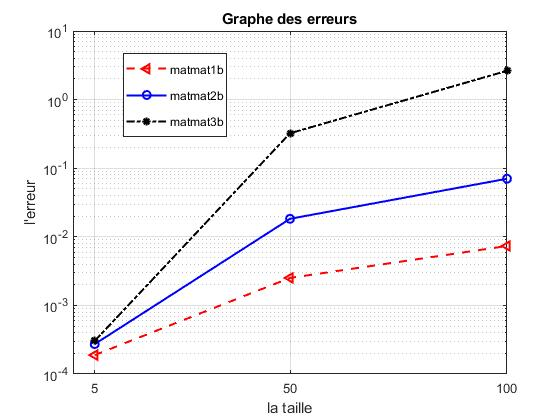
\includegraphics[scale=0.60]{graphe.jpg}~\\

\textbf{Analyse des resultats}\\

les trois algorithmes ont une une complixité differentes, le produit matrice-matrice de l'algorithme matmat3b qui déroule 3 boucle à une complixité cubique et la l'agorithme matmat2b à une complixité quadratique.\\

Les mesures de temps que nous avons fait pour les 3 algorithmes et pour les differentes taille, nous montre toujour que l'algorithme matmat1b qui a une complixité lineaire est le plus rapide. 
 
\chapter{TD/TP 3 Calcul Numérique Résolution de système linéaire}
\section{Exercice 1 TP Système Triangulaire}

Les méthodes directes reposent sur une décomposition de la matrice $A$ en $A = LU$ où $M$ est facile à inverser (triangulaire ou orthonormale) et $N$ est triangulaire. On aura donc
\begin{center}
$Ax = b \Leftrightarrow LUx = b \Leftrightarrow $ $\left\{\begin{array}{l} Lx=b \\ Ux=y\end{array}\right.$
\end{center}
Il faut donc savoir résoudre le système Ax = b lorsque A est triangulaire inférieure (ou supérieure).


Dans cet exercice nous allons voir les deux methodes de resolution des systémes triangulaire, la methode de remontée et de descente.\\

1. L'algorithme de la resolution par remonte : $usolve$ 

\begin{lstlisting}
function [x]= usolve(U,b)
 n = size(U,1);
 x = zeros(n);
 x(n) = b(n)/U(n, n);
 for i = n-1:-1:1
  x(i) = (b(i) - U(i, (i+1):n)*x((i+1):n))/U(i,i);
 end
endfunction
\end{lstlisting} 
         
2. L'algorithme de la resolution par remonte : $lsolve$ 

\begin{lstlisting}
function [x]= lsolve(L,b)
 n = size(L,2);
 x = zeros(n);
 x(1) = b(1)/L(1, 1);
 for i = 2:n
 x(i) = (b(i) - L(i, 1:(i - 1))*x(1:(i - 1)))/L(i, i);
 end 
endfunction 
\end{lstlisting}          
 
3. Test et validation des algorithme\\

Nous allons utiliser les deux fonctions \textbf{tril()} et \textbf{triu()} qui permettant d'extraire une matrice triangulaire inférieur ou supérieur.

\textbf{usolve :}\\

\begin{lstlisting}
 -->A
A  = 

0.7560439   0.6653811   0.685731      
0.0002211   0.6283918   0.8782165      
0.3303271   0.8497452   0.068374
\end{lstlisting} 

\begin{lstlisting}
 -->U=tril(A)
U  = 

0.7560439   0.          0.      
0.0002211   0.6283918   0.      
0.3303271   0.8497452   0.068374
\end{lstlisting} 

\begin{lstlisting}
-->b=A*xex 
b  = 

1.3377668
1.0127856
0.5407226
\end{lstlisting} 

\begin{lstlisting}
-->usolve(U,b)
ans  =

1.7694302
1.6117104
7.9083027
\end{lstlisting} 

\textbf{lsolve :}\\

\begin{lstlisting}
-->L=triu(A)
L  = 

0.7560439   0.6653811   0.685731 
0.          0.6283918   0.8782165
0.          0.          0.068374 
\end{lstlisting} 

\begin{lstlisting}
-->lsolve(L,b)
ans  =

1.7694302
1.6117104
7.9083027
\end{lstlisting}

\end{document}